\section{Fairness definitions}

\begin{frame}
  \frametitle{Fairness}
  What is it?
  \begin{itemize}
  \item<2-> \alert{Meritocracy}.
  \item<3-> Proportionality and representation.
  \item<4-> Equal treatment.
  \item<5-> \alert{Non-discrimination}.
  \end{itemize}
\end{frame}


\begin{frame}
  \frametitle{Meritocracy}
  
  \uncover<2->{
    \begin{example}[College admissions]
      \begin{itemize}
      \item Student $A$ has a grade 4/5 from Gota Highschool.
      \item Student $B$ has a grade 5/5 from Vasa Highschool.
      \end{itemize}
    \end{example}
  }
  \uncover<3->{
    \begin{example}[Additional information]
      \begin{itemize}
      \item 70\% of admitted Gota graduates with 4+ get their degree.
      \item 50\% of admitted Vasa graduates with 5 get their degree.
      \end{itemize}
    \end{example}
  }
  \uncover<4->{We still don't know how a \alert{specific} student will do!}
  \begin{block}<4->{Solutions}
    \begin{itemize}
    \item<5-> Admit \alert{everybody}?
    \item<6-> Admit \alert{randomly}?
    \item<7-> Use \alert{prediction} of individual academic performance?
    \end{itemize}
  \end{block}
  


\end{frame}

\begin{frame}
  \frametitle{Proportional representation}
  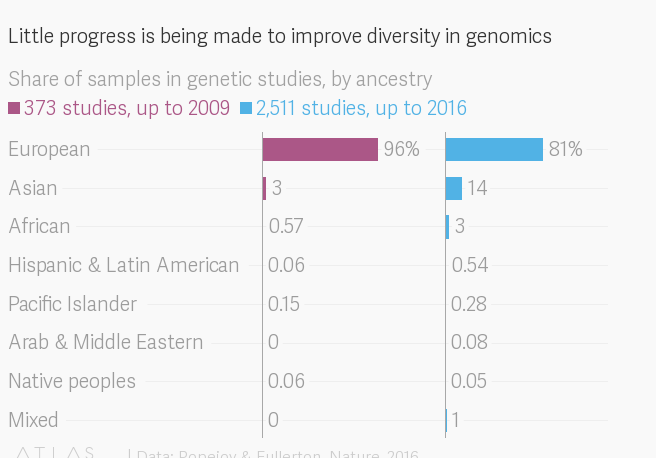
\includegraphics[width=\textwidth]{../figures/genomics-diversity}
  \url{https://qz.com/1367177/}
\end{frame}



\begin{frame}
  \frametitle{Hiring decisions}
  \begin{columns}
    \begin{column}{0.5\textwidth}
      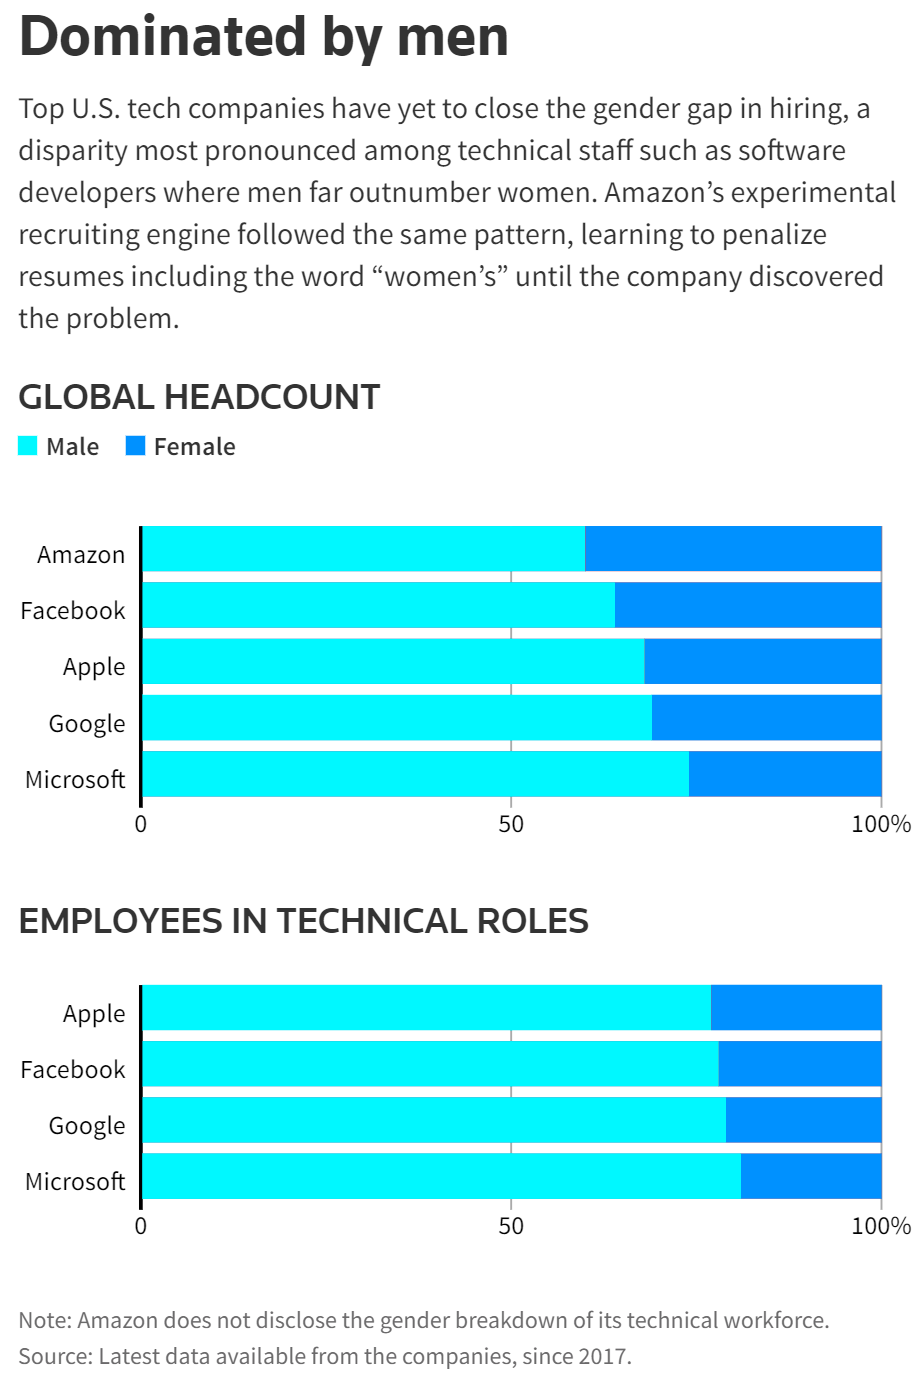
\includegraphics[height=\textheight]{../figures/cmu-headcount}
    \end{column}
    \begin{column}{0.5\textwidth}
      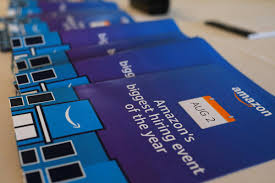
\includegraphics[width=\columnwidth]{../figures/amazon-hiring}
      \\
      
\includegraphics[width=\columnwidth]{../figures/recruitement-automation}
    \end{column}
  \end{columns}
\end{frame}

\begin{frame}
  \frametitle{Fairness and information}
  \begin{example}[College admissions data]
    \begin{table}[H]
      \begin{tabular}{l|r|r}
        School & Male  & Female\\
        \hline
        A & 62\% & 82\%\\
        B & 63\% & 68\%\\
        C & 37\% & 34\%\\
        D & 33\% & 35\%\\
        E & 28\% & 24\%\\
        F &  6\% &  7\%\\
        \hline
        \emph{Average} & \emph{45\%} & \emph{38\%}
      \end{tabular}
    \end{table}
  \end{example}
\end{frame}

\begin{frame}
  \centering
  {\Huge The US bail system}
\end{frame}

\begin{frame}
  \frametitle{Bail decisions}
  \centering

  \begin{columns}
    \begin{column}{0.5\textwidth}
      \begin{tikzpicture}
        \node at (-1,2) (person)
        {
\includegraphics[width=0.2\columnwidth]{../figures/zuckerberg}};
        \node at (0,0) (judge) {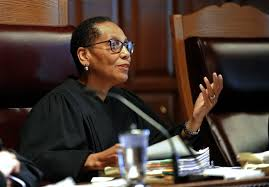
\includegraphics[width=0.3\columnwidth]{../figures/judge}};
        \draw[->] (person) -- (judge);
        \uncover<2->{
          \node at (-2,-2) (jail) {
\includegraphics[width=0.3\columnwidth]{../figures/jail}};
          \draw[->] (judge) -- (jail);
        }
        \uncover<3->{
          \node at (2,-2) (bail) {
\includegraphics[width=0.3\columnwidth]{../figures/bail}};
          \draw[->] (judge) -- (bail);
        }
        \uncover<4->{
          \node at (-2,-4) (trial) {
\includegraphics[width=0.3\columnwidth]{../figures/trial}};
          \draw (jail) -- (trial);
        }
        \uncover<5->{
          \draw (bail) -- (trial);
        }
        \uncover<6->{
          \node[label=$y_2$] at (2,-4) (arrest) {
\includegraphics[width=0.3\columnwidth]{../figures/handcuffs}};
          \draw (bail) -- (arrest);
        }
      \end{tikzpicture}
    \end{column}
    \begin{column}{0.5\textwidth}
      \includegraphics<7>[width=0.8\columnwidth]{../figures/judge-fairness}

    \end{column}
  \end{columns}

  \note<1>{Let us begin with a simple example. In the US system of justice, an accused is presented before a judge. The accused has some observable features x, as well as some possibly sensitive features z such as ethnicity or gender.}
  \note<2>{ Based on what the judge sees, she uses a policy pi to make a decision. Should the defendant be kept in jail until trial?}
  \note<3>{Or should they be let go?}
  \note<4>{If they are kept in jail, then they almost invariably go to trial.}
  \note<5>{They may also go to trial if they are freed...}
  \note<6>{But they may also flee or commit another crime.}
  \note<7>{Typically, the judge makes the decision by weighing the risk against a utility function that measures the cost of keeping an innocent in prison versus the cost of them committing another crime.}
\end{frame}

\begin{frame}
  \frametitle{The USA COMPAS System\footnote{Pro-publica, 2016}}
  Assigns a \alert{risk score} to defendant.
  \begin{figure}[H]
    \begin{columns}
      \begin{column}{0.5\textwidth}
        \centering
        \def\svgwidth{.95\columnwidth}
        \input{../figures/risk-scores-black.pdf_tex}
        Black
      \end{column}
      \begin{column}{0.5\textwidth}
        \centering
        \def\svgwidth{0.95\columnwidth}
        \input{../figures/risk-scores-white.pdf_tex}      
        White
      \end{column}
    \end{columns}
    \label{fig:risk-bias}
    \caption{Apparent bias in risk scores towards black versus white defendants.}
  \end{figure}
\end{frame}


\subsection{Group fairness and conditional independence}
\begin{frame}
  \only<1>{
    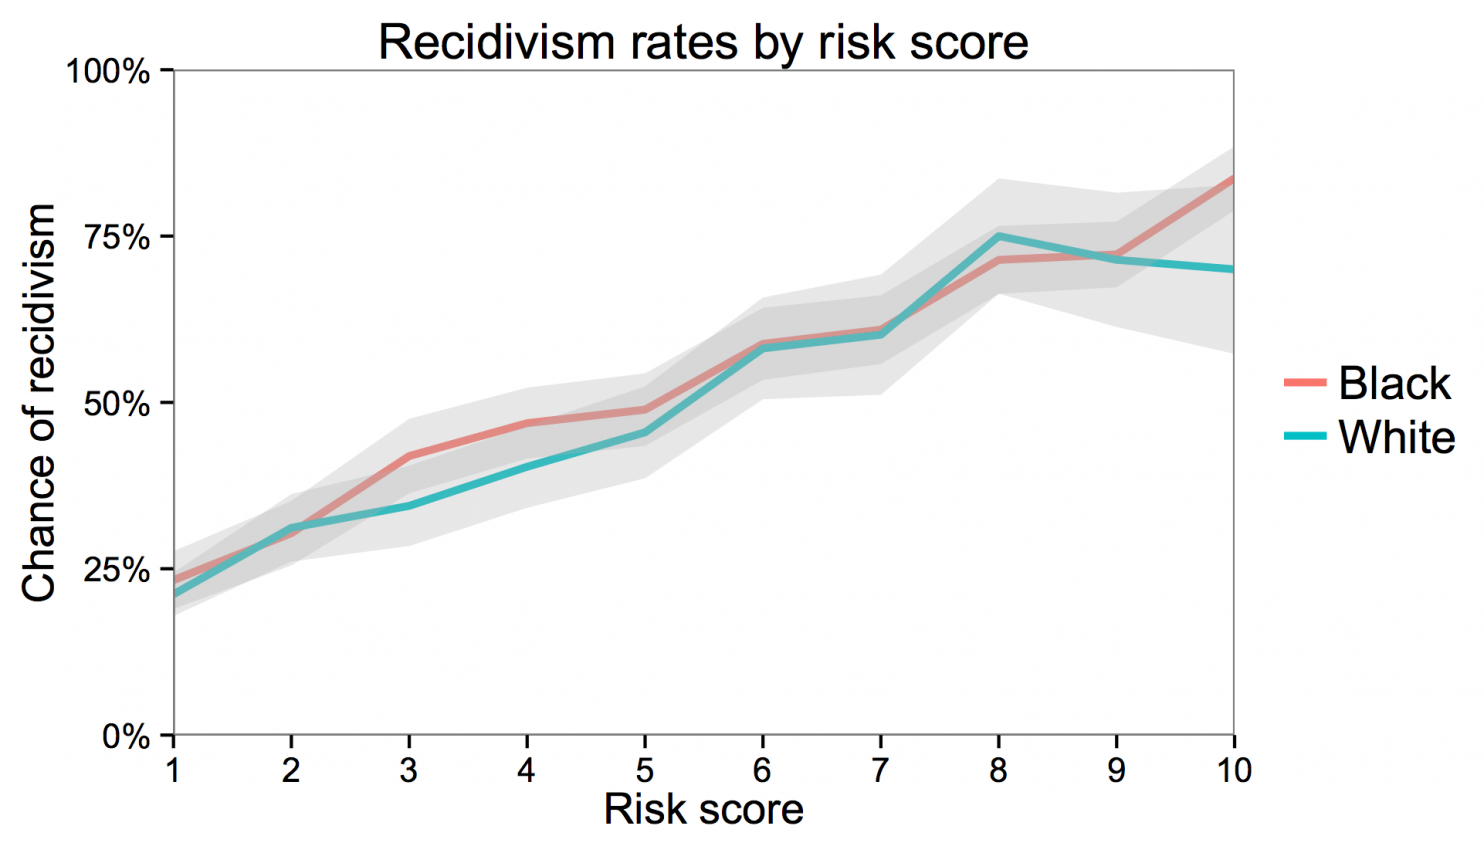
\includegraphics[width=\columnwidth]{../figures/imrs}
    \\\scriptsize{Washington Post, 2016}
  }
  \only<2>{
    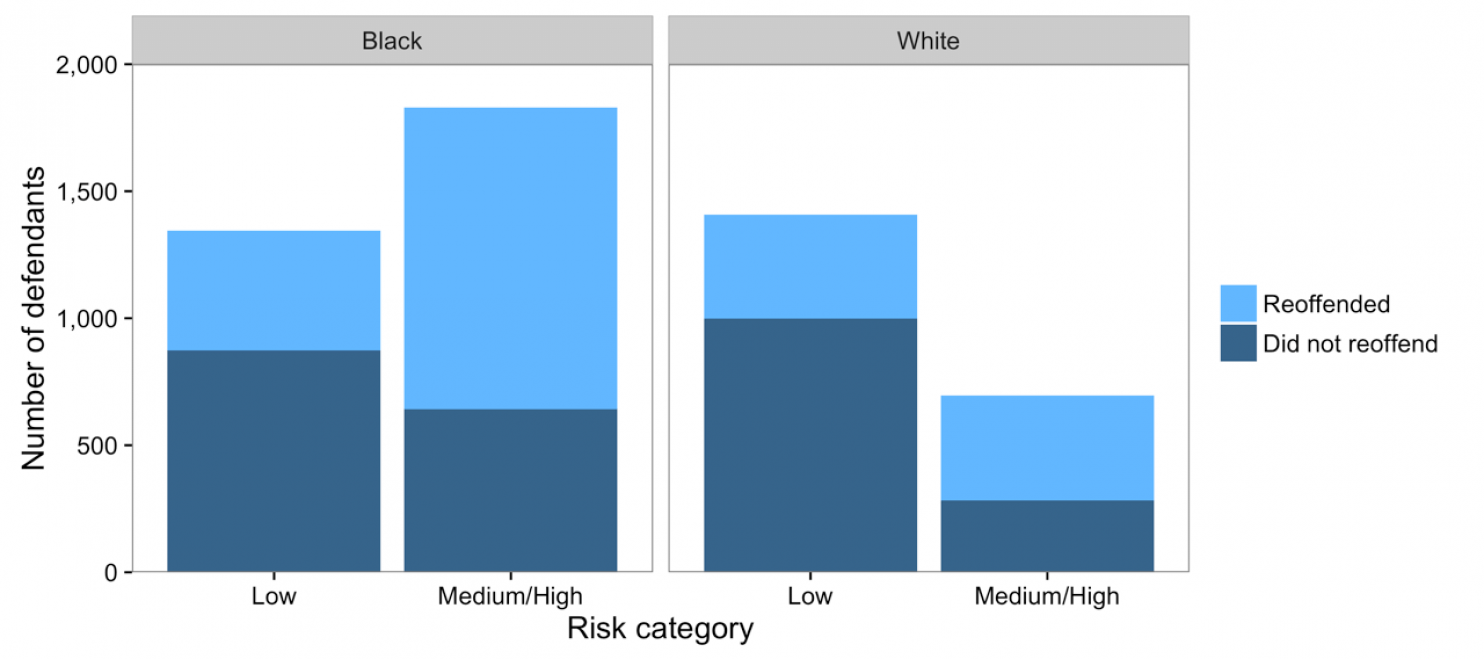
\includegraphics[width=\columnwidth]{../figures/imrs-risk}
    \\\scriptsize{Pro-publica, 2016}
  }
\end{frame}

\section{Public attitudes}
\begin{frame}
  \centering
  {\Huge Public attitudes towards fairness}
\end{frame}
\begin{frame}
  \frametitle{Lending\footnote{Saxena et al, 2018 -- arxiv:1811.03654}}
  \centering
  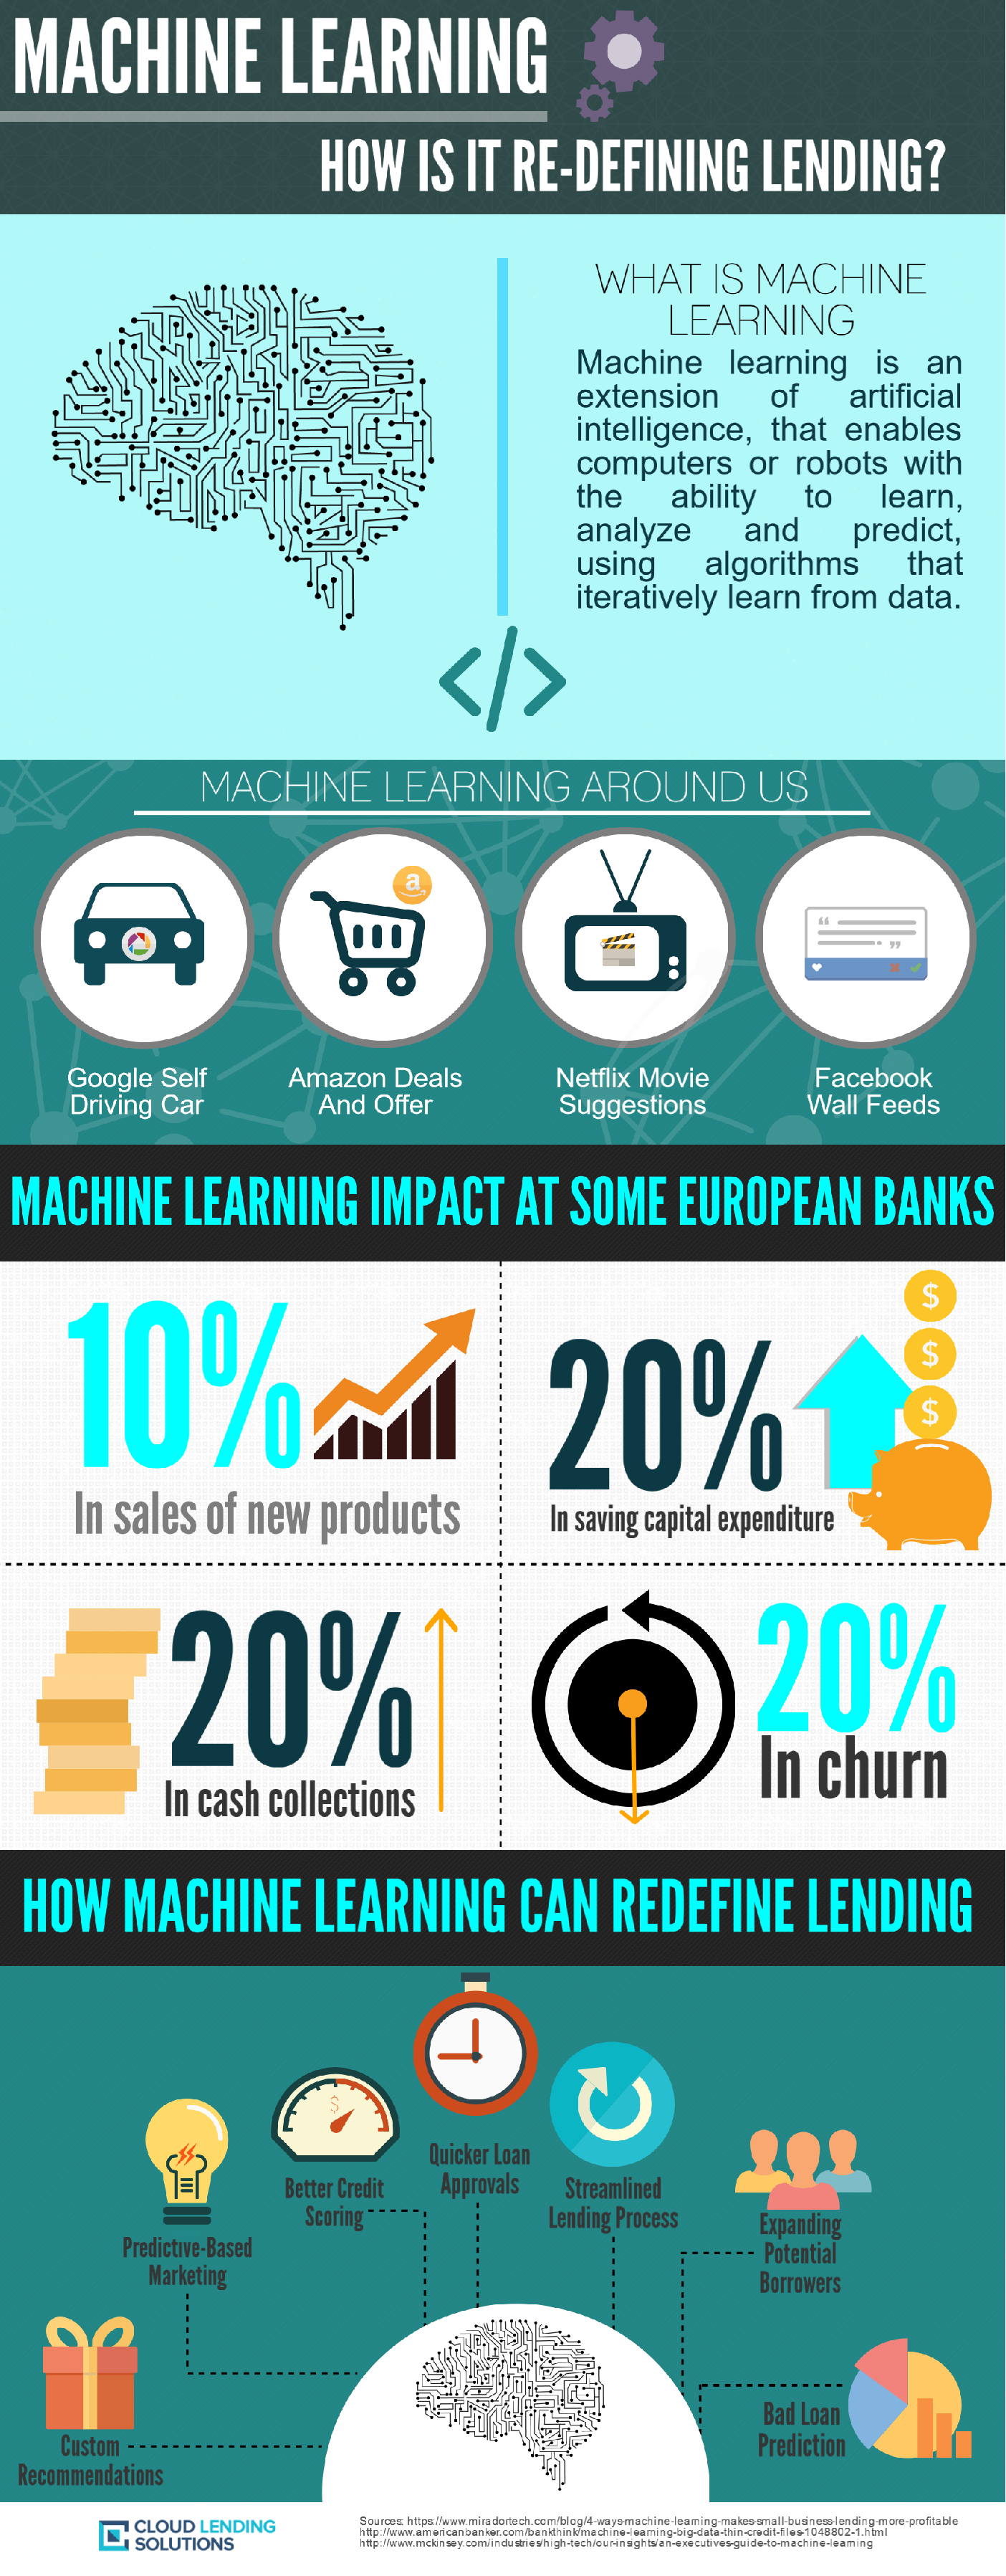
\includegraphics[width=0.5\textwidth,clip = true, trim=0 0 0 42.5cm]{../figures/lending.pdf}

  \begin{block}{Setting}
    \begin{itemize}
    \item Attribute: Repayment rate.
    \item Sensitive attribute: race, gender.
    \item Decision: Loan amount.
    \end{itemize}
  \end{block}
\end{frame}

\begin{frame}
  \frametitle{Studies}
  Given two people with different \alert{estimated} repayment rates:
  \only<1>{
    \begin{itemize}
    \item A: 55\%
    \item B: 50\%
    \end{itemize}
  }
  \only<2>{
    \begin{itemize}
    \item A: 70\%
    \item B: 40\%
    \end{itemize}
  }
  \only<3>{
    \begin{itemize}
    \item A: 90\%
    \item B: 100\%
    \end{itemize}
  }
  \only<4>{
    \begin{itemize}
    \item A: 100\%
    \item B: 20\%
    \end{itemize}
  }
  \begin{block}{Decisions}
    \begin{itemize}
    \item All money to the person with highest payback rate.
    \item Equally split money.
    \item Proportionally allocate money.
    \end{itemize}
  \end{block}
  \uncover<5>{
    \begin{block}{Results}
      \begin{itemize}
      \item No sensitive information: Proportionality.
      \item Race and gender: Proportionality, but more supportive of allocating all to black with high repayment rates.
      \end{itemize}
    \end{block}
  }
\end{frame}


\begin{frame}
  \frametitle{Scenario dependence\footnote{Srivastava et al, 2019 -- arXiv:1902.04783}}

  \begin{tabular}{l|l|l|l}
    Algorithm & Accuracy & Acc. Females & Acc Males\\
    \hline
    A & 94\% & 89\% & 99\% \\
    B & 91\% & 90\% & 92\% \\
    C & 86\% & 86\% & 86\%
  \end{tabular}

  \only<1>{
    If this is a diagnostic test for \alert{skin cancer}, which algorithm is the most ethical to use?
  }
  \only<2>{
    If this is a diagnostic test for \alert{flu}, which algorithm is the most ethical to use?
  }
\end{frame}

\begin{frame}
  \frametitle{Conclusion}
  \begin{itemize}
  \item Multiple (incompatible) definitions of fairness.
  \item Fairness is hard to measure.
  \item The effect of more fair policies on society is harder to predict.
  \item Computer scientists, statisticians, economists and law professionals must work closely with the public, industry and civil servants.
  \end{itemize}
\end{frame}
%%% Local Variables:
%%% mode: latex
%%% TeX-master: "fairness-presentation-vetenskap"
%%% End:
